% !TeX encoding = UTF-8

\documentclass{LTHtwocol} % Use this when you work on your report.
% \documentclass[final]{LTHtwocol} % Use this for the final version.
                                   % It will remove page numbers and
                                   % markers for overfull boxes.
                                   % There really shouldn't be any of those anyway.

\usepackage[utf8]{inputenc}        
\usepackage{amsmath,amssymb,graphicx}
%\usepackage{hyperref} 
%\usepackage{GroupC-bibliography.bib}

% Useful commands for easy figure and table referencing
\newcommand{\figref}[1]{Figure~\ref{#1}}
\newcommand{\tabref}[1]{Table~\ref{#1}}

\addbibresource{GroupC-bibliography.bib}
%\bibliography{GroupC-bibliography.bib}

% Document begins here
\begin{document}
\begin{frontmatter}
\title{F1/tenth car} % Title of the project.
                      % Note that all reports are in English,
                      %so that our international students can read them.

\author[Rebeca]{Rebeca Homssi}
\author[Albert]{Albert Anderberg}
\author[Josiah]{Josiah Wong}


\email[Rebeca]{tpi14rho@student.lu.se}
\email[Albert]{elt14aan@student.lth.se}
\email[Josiah]{jo7036wo-s@student.lu.se}

%\begin{abstract}
%    The abstract should be a 200--250 word compact description of your project. What was the objective? Which methods did you use? What was the (main) result?
%\end{abstract}

\end{frontmatter}

% Stick to the proposed structure below. Add \subsections{} as appropriate.
% This file compiles on the Automatic Control Department system by typing the
% following into the terminal (while in the directory of the file, and with all
% other files belonging to the template untouched):
% > pdflatex template        
% > biber template
% The first line compiles the .tex file. The second line generates the
% bibliography. Once this is done, you may need to run the first line 1-2
% additional times, for the system to get all cross references right in the
% produced pdf output.

\section{Introduction}
%Here you introduce the project. What is the background? What project do you aim at solve? References to prior work? If the project makes a positive or negative environmental, or other solitary, impact, describe it here. Are there any ethical considerations? You might want to reference relevant literature, e.g. \cite{openclosed2, Hellerstein2004, Yun2015}. A general \LaTeX\ guide is available at \cite{latexwiki}. 

Self driving cars and automation of cars is a hot topic today. Every car company in the world races in the development of cars to be the first to launch a completely self driving car that can handle every possible situation on the road. Today the development has come far and there is some cars on the market that are partly self driving.

In this project we will work with the F1/tenth car which is 1/10 size of a formula 1 car. The car is shown in figure \ref{fig:f1tenthcar} below. The aim of this project is to learn how to model, control and design the car to be able to make it self-driving. The goal of this project is to create a controller and a path planning model that can navigate the f1/tenth car through a known path keeping a certain distance to the wall and avoiding obstacles that can appear on the way. The model and design will be based on feedback from the LIDAR sensor and the IMU. At last we will develop the path planning model to be able to navigate the car to overtake another car.

\begin{figure}[h]
	\centering
	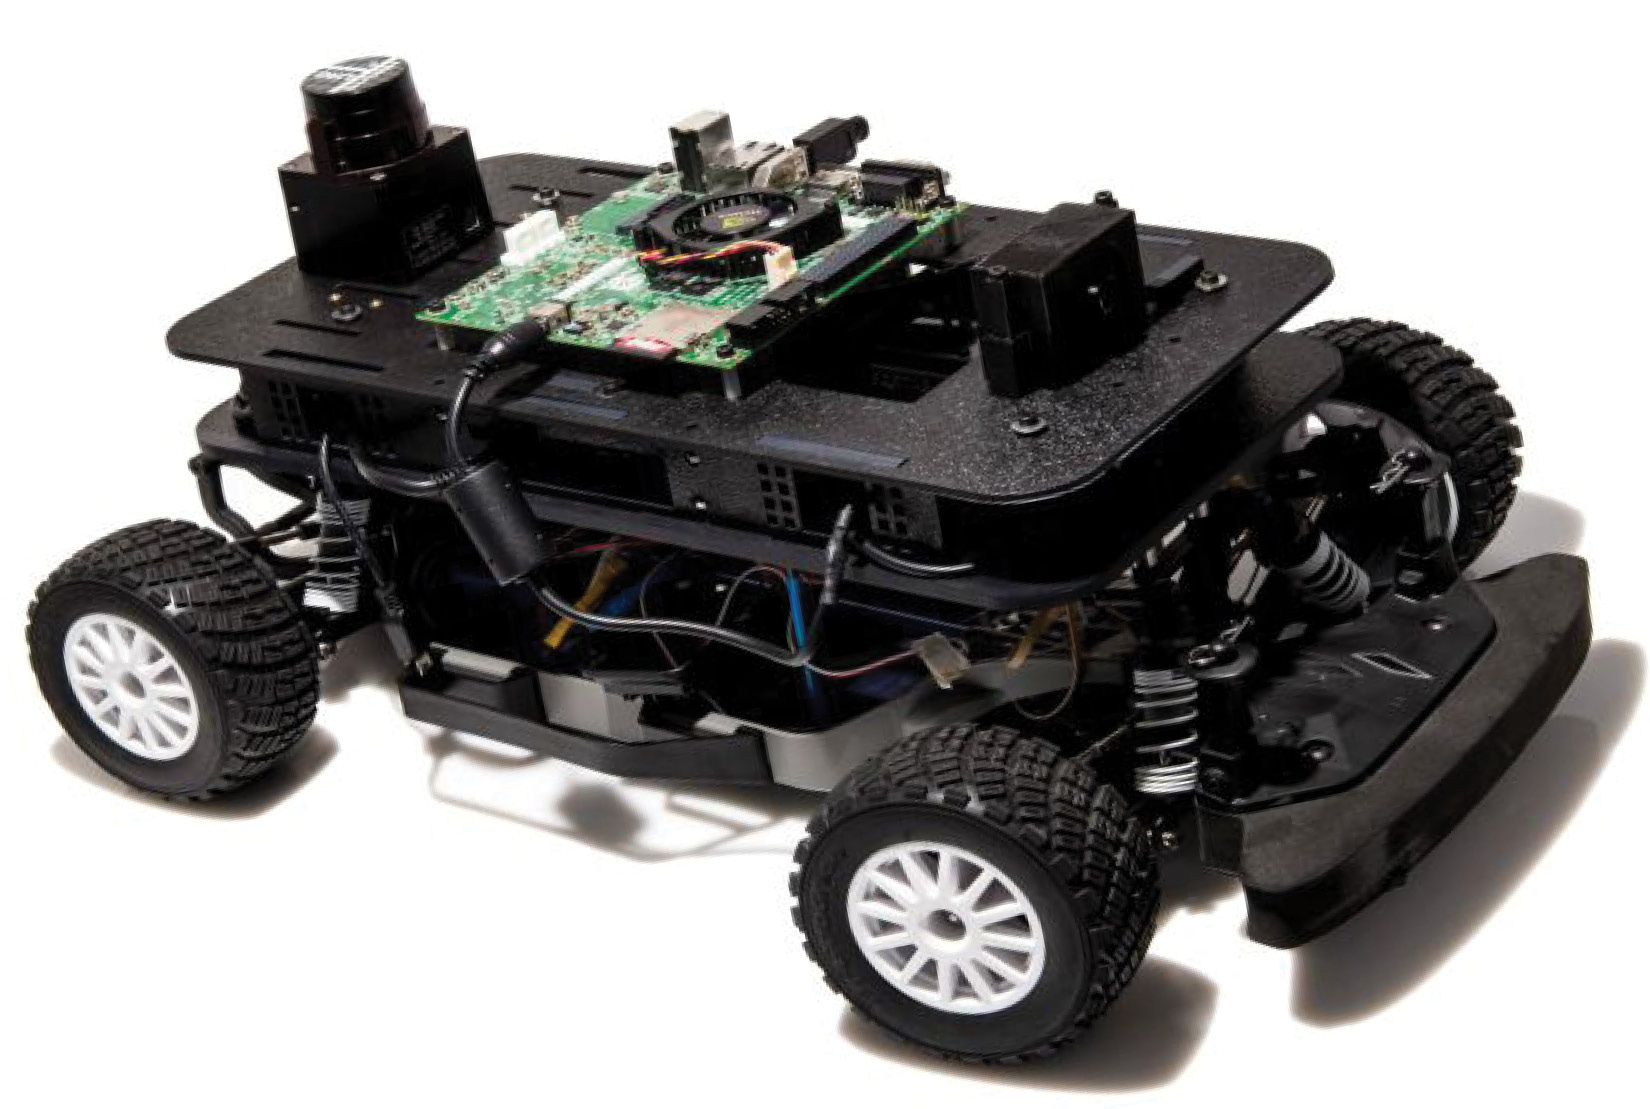
\includegraphics[width=0.7\columnwidth]{images/f1tenthcar}
	\caption{Picture of the f1/tenth car used in this project. In the front is the camera and in the back is the Lidar sensor. Image courtesy of the f1tenth project, \cite{teensy_schematic}.}
	\label{fig:f1tenthcar}
\end{figure}

\subsection{Background and Prior work} 
In 1977 the first automated car that could track streets were launched in Japan. Since then many companies and organizations has developed prototypes with different levels of automatic driving. The level of automation can be described on a 0-5 scale, where level 5 is completely self driving car with no need of human steering. But the development has gone slowly until year 2012 when states in US started to allow testing of automatic cars on public roads.  Today there is over 100 self-driving cars on the public streets in the US \cite{wikiSelfDrivingCar}. In 2017 in Gothenburg, Sweden, Volvo Cars launched a project where 100 households were picked out to use Volvos new self-driving cars, level 4, in there daily life \cite{volvoCars}. Today no car has reached level 5 in automation.

Creating a self driving car is a technical challenge. There are many sensors and control systems needed to be able to get accurate data from the surroundings. Typical sensors that are used is Lidar, stereo vision, GPS and IMU. Based on the information from the sensors the car should make an accurate localization of itself, its surroundings and create a path plan for the car to follow. The path plan tries to find the safest, fastest and most beneficial way from one point to another. There has been many studies on how to design the path planning model. In the master thesis "Motion Planning using Positively Invariant Sets on a Small-Scale Autonomous Vehicle" the authors used invariant sets to create a path planning model which could safely navigate a small car to overtake another car \cite{masterthesis}. Further in the article " A Survey of Motion Planning and Control Techniques for Self-driving Urban Vehicles" a thorough comparison has been made between 11 different path planning methods. The article  shows that the different methods are well developed but should be used with a feedback controller that stabilizes the obtained path \cite{motionPlanningArticle}.


% If we need more text I could write about benefits and disadvantages of self-driving cars.



\section{Modeling}
%Here you present the modeling approach and publish your model.  The idea is, however, that another group with your background should be able to reproduce your work -- this goes not only for the modeling aspect.If you use equations, make sure they are all numbered and referenced, as \eqref{eq:formula}. Equations are parts of the text. If they end a sentence, they should end with a dot. If they end a clause, they should end with a comma. See \cite{mathslatexwiki} for a tutorial on typesetting maths.

% describe input, output
% what commands are sent to the car 

Control of the car was modeled as a MISO system, with the two inputs being PWMs sent to the speed controller and steering servo motor, and the single output being a weighted combination of the car's distance from the (right-hand side) wall and (scaled) angle relative to the wall. The resolution of the PWM was sufficient to control the (min, max) = (-100,100) values of the steering and speed to within 0.5 incremental steps.

While the final control system was relatively straightforward and required minimal structured modeling, it is important to note that our system's success was based upon a few critical assumptions, namely:

\begin{itemize}
	\item The car is an inherently stable system
	\item Inputted voltage (PWM) is proportional to resulting speed
	\item Non-linearities related to steering may be neglected
\end{itemize}

The first assumption is necessary for the latter two assumptions to even be considered, for a stable system is much easier to heuristically tune compared to an unstable system. The second and third assumptions justify our usage of a simple PID controller, for the scope of our system does not require near-instantaneous response times that would necessitate a more complex, robust modeling of the car's steering (angular) dynamics.

\section{Electro-Mechanics}
The car is based on version 1 of the f1/10 car from the f1tenth project. Some of the more important parts can be seen in the list below and a short description can be seen in the following sections.

% Rewrite the above section and insert picture of our car

\begin{itemize}
	\item Electric speed control
	\item Steering servo
	\item Teensy control board
	\item NVIDIA Jetson TK1 developer kit
	\item Hokuyo UST-10LX Lidar
	\item SparkFun 9DoF Razor IMU M0
\end{itemize}

\subsection{Electric speed control and steering servo}
The car is based on the Traxxas 1/10th Car platform which is a normal remote controlled car. However since our project and the f1tenth projects goal is to control it from a computer some modifications has to be made. The standard configuration contains three different parts, the radio transceiver, the steering servo and the electric speed controller, hereafter shortened to ESC. In the default configuration the steering servo and the ESC is directly connected to the radio transceiver which generates the control signals. The control signals are pulse width modulated signals where different duty cycle represents different steering angles and different velocities. A control board is inserted between the radio transceiver and the actuators that will generate the required pwm signals.

\subsection{Teensy control board}
The control board is based on the teensy micro controller. \figref{fig:teensy_schematic} contains the very simple schematic for the control board. The different three pin connectors all contains the same signal types, VCC, GND and a pulse width modulated signal. To the connectors JP1 and JP2 the ESC and steering servo is connected respectively. To connector JP3 and JP4 the original control signals from the transceiver is connected. The switch S1 can be used to switch which control signal is used, either the one from the radio transceiver or the one generated by the teensy board.

Not included in the schematic in \figref{fig:teensy_schematic} is the USB connection between the Teensy and the Jetson board. To generate the pwm signals the 16-bit timers on the Teensy is used and the pwm signals are generated by the Teensys hardware. The required control signals are received from the Jetson through the emulated serial port over the USB connection.

\begin{figure}[b]
	\centering
	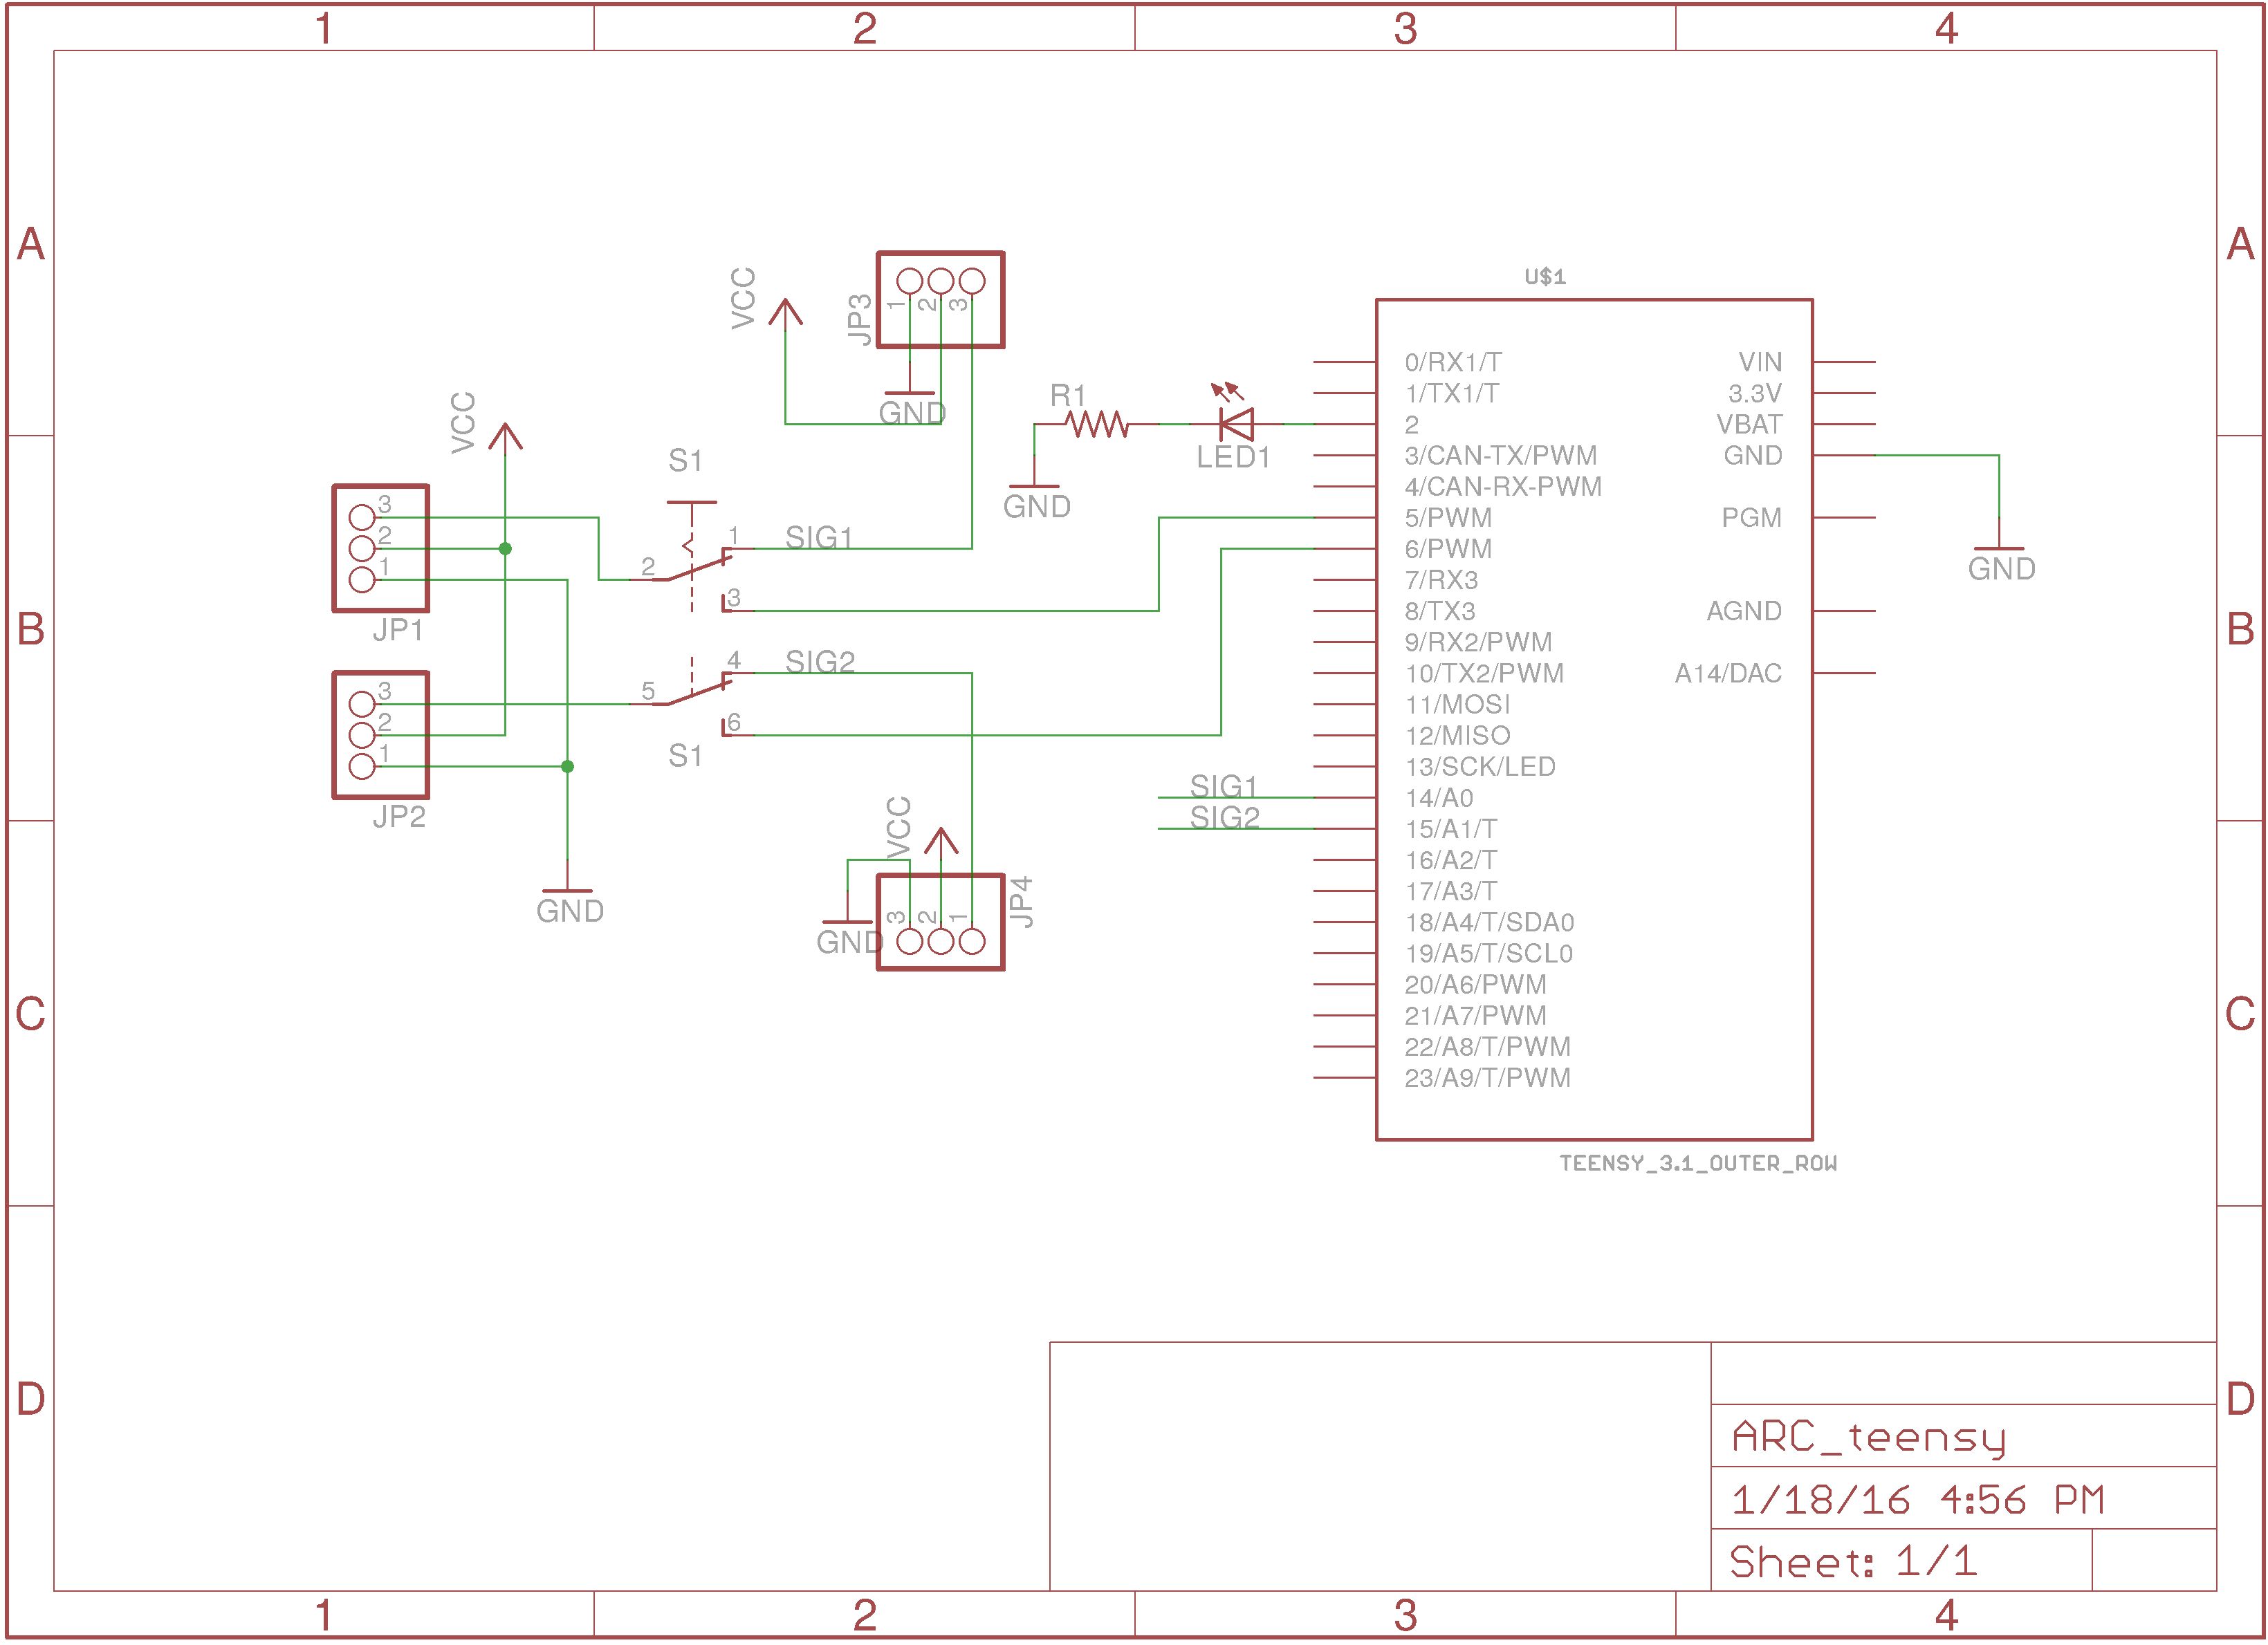
\includegraphics[width=0.7\columnwidth]{images/teensy_schematic}
	\caption{Electrical schematic for the control board based on the teensy micro controller. Image courtesy of the f1tenth project, \cite{teensy_schematic}.}
	\label{fig:teensy_schematic}
\end{figure}

\subsection{NVIDIA Jetson TK1 developer kit, Lidar and IMU}
The so to say brain of the car is the NVIDIA Jetson TK1 developer kit, hereafter simply refereed to as Jetson. The Jetson runs Ubuntu 14.04 and ROS(Robot Operating System) Indigo. The IMU and the Teensy controller board are connected through USB to the Jetson. The Lidar is connected to the jetson through a ethernet connection. Since the onboard ethernet connection is already in use by the wireless accesspoint, Ubiquiti PicoStationM2HP, a separate USB to ethernet adapter is used to connect the lidar. Since two ethernet interfaces are used they have to be bridged so that the lidar is accessible from the rest of the network. This bridge runs and is configured in the Jetson.


\section{Control}
%This is the core of your report. What controller structure and strategy did you use? How did you come up to this choice?
At the high level, the Hector SLAM algorithm leveraging the on-board LIDAR was utilized to localize the car while mapping its environment. On an implementation level, a simple single-channel PID controller was determined to be sufficient for stabilizing and maintaining the car's intended trajectory parallel to the wall. On the software side, the ROS platform was used to simultaneously run the path planning algorithms and trajectory controllers.

\subsection{Software structure/design/implementation}
Software in ROS is divided into different packages. These packages could be local packages written by the user or external packages written by the ROS community that has been downloaded either as a part of the standard ROS installation or separately by the user. A package can contain any number of nodes which contains the code that is running. A package can also contain launch files that describes how and which nodes should be run. A launch file is not limited to only run nodes from the same package but can run any node that is available in the ROS environment. Communication between nodes are done using topics. A node can subscribe to a topic to receive messages published to this topic by another node. A message can contain different data dependent on which message definition is used. A simple message can consist of a single boolean, such as an on/off switch, but also more complicated data such as arrays containing distance measurements from a lidar.

\begin{figure}
	\centering
	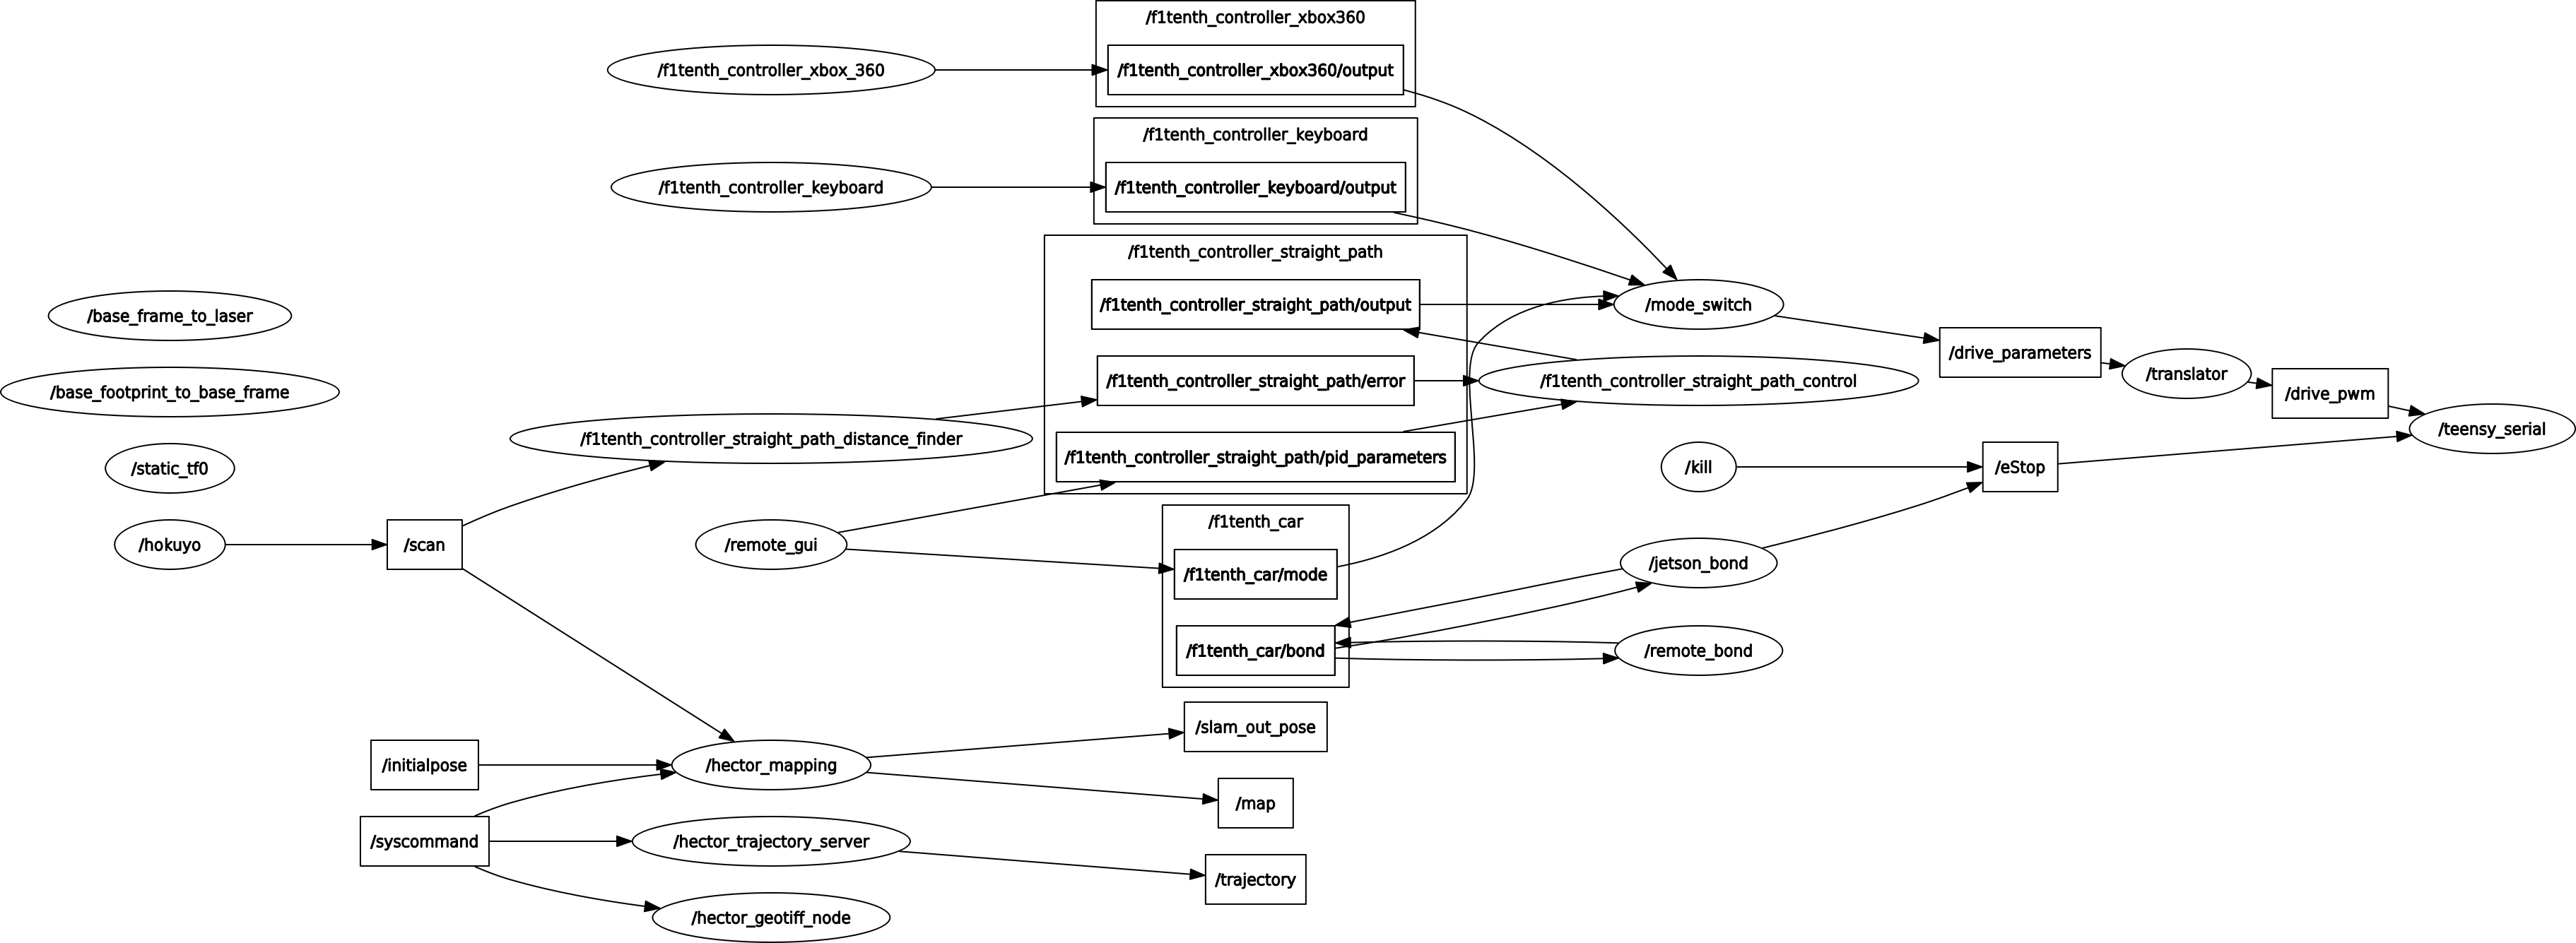
\includegraphics[width=0.7\columnwidth]{images/rosgraph}
	\caption{rosgraph}
	\label{fig:rosgraph}
\end{figure}

ROS also has native network support which means that different nodes can be run on different hosts. To be able to use multiple hosts one host has to be designated as the master. The other nodes then has to be configured on where to find the master host and then nodes can be run in the same way as they were running on the same machine. There are however some limitations when running on multiple hosts, such as that any node that is communicating with hardware has to be running on the same host as the hardware is connected to.

The code for this project can be divided into three different bundles of code, which can consist of multiple packages. The first bundle is the code running on the Jetson which consists of all the nodes that interact with hardware and most of the controller nodes. The second bundle is the nodes running on the remote computer, such as a laptop. A graphical user interface and visualization tools are part of this bundle. The third bundle could be seen as a part of the second as it only contains the emergency stop code for the remote system. There is however an advantage to keep this functionality as separate as possible from the rest of the remote control since if the remote control crashes or stops unexpectedly the remote emergency stop should still be working as intended.

Using the \texttt{rqt\_graph}\cite{rqt_graph} utility the image in \figref{fig:rosgraph} can be generated when the software is running. Generally data/information flows from left to right in the figure. At the far right side of the graph the \texttt{/teensy\_serial} node can be found. This node is responsible for the communication with the teensy control board and subscribes to the \texttt{/eStop} and \texttt{/drive\_pwm} topics. The \texttt{/kill} node is emergency stop node running on the remote computer and publishes to the \texttt{/eStop} topic. The second publisher on the \texttt{/eStop} topic is the \texttt{/jetson\_bond} node which runs on the Jetson. Together with the complimentary \texttt{/remote\_bond} node, running on the remote computer, these nodes keep track of the connectivity between the different computers using a heartbeat signal. If the connection is lost the \texttt{/jetson\_bond} node will engage the emergency stop by publishing the value true on the \texttt{/eStop} topic.

Going up the other branch we pass through the \texttt{/translator} node and find the \texttt{/mode\_switch} node. The \texttt{/translator} nodes objective is to translate the control values from the mode switch, which are in the range -100 to 100, to the values used by the Teensy board. The \texttt{/mode\_switch} nodes objective is to, as the name suggest, switch between different operating modes. The different operating modes could be manual control, such as the \texttt{/f1tenth\_controller\_keyboard} node, or automatic control, such as the \\ \texttt{/f1tenth\_controller\_straight\_path\_control} node. One mode that is not visible in the graph is the off mode which simply is used to turn of all actuators. The mode switch is controlled by the remote graphical user interface using the \texttt{/f1tenth\_car/mode} topic. From the graphical user interface it is also possible to change the parameters for the straight path controller. The straight path controller is divided into two nodes, \texttt{/f1tenth\_controller\_straight\_path\_control} and \texttt{/f1tenth\_controller\_straight\_path\_dist\_finder}, which together finds the distance to the wall using lidar data from the \texttt{/scan} topic and controls the car so that the distance to the wall is kept constant. The second subscriber to the \texttt{/scan} topic is the \texttt{/hector\_mapping} node. This node together with the other hector nodes is used to build the map and current trajectory.

\subsection{Sensors and measurement unit}
One of the sensors used on the cars is the Lidar sensor. The Lidar sensor sends out pulsed laser light to measure distances. In the beginning of the project the Lidar was used to measure the distance to a wall, to make the controller keep a certain distance to the wall. But going further in this project the Lidar sensor is used not only to measure distance to a certain wall but also to map the distances to walls and objects around the car. Using the data from the Lidar a map of the environment can we created. More about how this is done in section \ref{sec:Hector}.

%The second sensor is a camera ... 

The measurement unit used is the inertial measurement unit, IMU. The IMU measures and reports the speed and acceleration of the car. For the moment the IMU is barely used but when the car is able to drive around freely in the basement or when the car is overtaking another car the IMU will become more important.

\subsection{Hector - SLAM} \label{sec:Hector}
Mapping out the environment while driving takes a lot of computation time but since we always will be driving the car in the basement we only need to create a map once of the environment and then use this map when driving. To be able to build up some sort of graphical view of the environment measurements obtained from the Lidar we use the \texttt{hector\_slam} package in ROS. In this package we have three nodes, the \texttt{hector\_mapping}, \texttt{hector\_geotiff} and the \texttt{hector\_trajectory\_server}. The \texttt{hector\_mapping} node uses simultaneous localisation and mapping, SLAM, to learn the map. The \texttt{hector\_geotiff} node saves the map and trajectories and the \texttt{hector\_trajectory\_server} saves the multiple coordinate frames over time, in ROS these are called \texttt{tf}.

The package start with a first scan of the environment and initial position. Then a small change in position is done before another scan is made. The two scans is matched and a new position of the car is estimated using these measurement. Continuing these process we will obtain a map of the environment. 
%hmm this should maybe be moved to result?
In figure \figref{fig:hectorMap} a map of the basement in the M-building can be seen. The map was obtained using the \texttt{hector\_slam} package described above. The green lines in the map is the driving path made when obtaining this map. 

\begin{figure} [h]
	\centering
	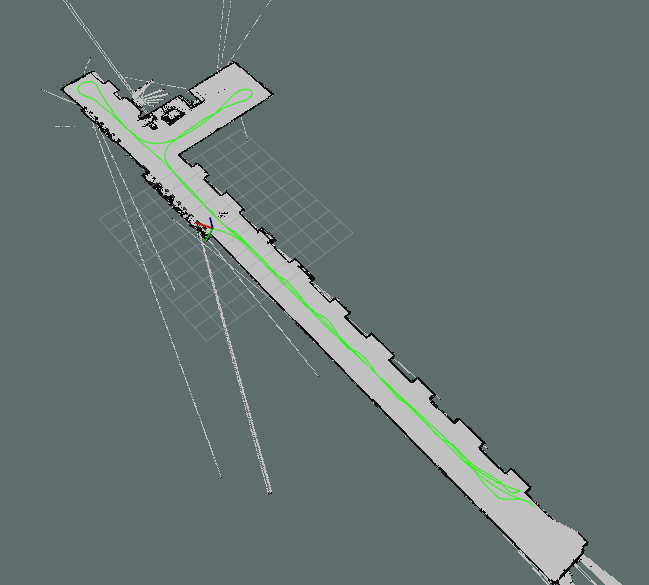
\includegraphics[width=0.7\columnwidth]{images/hectorMap}
	\caption{Map of the basement in the M building using hector\_slam package together with Lidar.}
	\label{fig:hectorMap}
\end{figure}

\subsection{Particle filter}
Now we have a map but to be able to use it we need to know the localization of the car in the map. This is done using a particle filter. The particle filter starts with a odometry pose and then add some Gaussian distributed noise to get a set of possible poses. A Lidar scan orientation is made and for each of the poses the correlation between the scan and the map from hector is computed. The pose with the highest correlation is chosen to be the position of the car. For each scan a position update is done.

%The filter updates around 30 times per second and have a result of around 100x the number of particles which result in good accuracy.

\subsection{Path Planning}
A three-step process will be implemented to overtake another car. At a high level, it can be seen as follows:

\begin{enumerate}
	\item Follow the other car at a set distance at the same speed
	\item Determine the "safe distance from wall" threshold required to safely pass the car
	\item If safe, execute a pre-designed trajectory
	\item Check for changes in other car's (straight) trajectory, and abort if detected
\end{enumerate}

The first step simplifies the path planning process by creating a standard "initial condition" upon which a specific trajectory planner may be designed. This will be achieved either by (a) a mounted webcam checking for a marker on the back of the other car, or (b) LIDAR detecting abnormalities within the pre-constructed static map of the environment. In either case, control signals will be sent to calibrate the car's orientation and distance relative to the other car.

The next step calculates the distance required to safely surpass the other car and avoid a collision with the forward-facing wall during execution. Given a pre-designed passing trajectory, it becomes a simple, relatively linear function proportional to the velocity of the other car.

Assuming the threshold distance value is met, the main car will execute a pre-designed trajectory to pass the other car. This is a justified decision, given the known dynamics and dimensions of the other car. This can be accomplished by providing localized and dynamic "waypoints" within the map for the car to follow and must pass with a certain velocity. 

Lastly, because the path planner assumes the other car remains at a fixed velocity and orientation (i.e.: straight driving), the main car must check for either changes in the other car's angular position relative to its own as well as increases in the other car's velocity, either of which will result in an abortion of the intended passing trajectory and "resetting" of the Algorithm to Step 1.

\subsection{Control}
For each time step, a two-channel PID controller will be implemented to achieve the various trajectories required in the above algorithm. One channel will control the steering, while the other will control the velocity. The steering controller values have been heuristically tuned to \textbf{\[k_p = X, k_i = Y, k_d = Z,\]} while tuning is yet to be done on the velocity controller. Because the voltage level input to a DC motor is proportional to its steady state speed, the PID velocity controller is expected to work with iterative tuning. Waypoints will be utilized to define the car's time-sensitive position and velocity states and serve as inputs to the controllers.

\section{Results}
To be done later.
\section{Discussion}
To be done later.

%Discuss the results and what you learned from the project.


% Prints cited references
\printbibliography


\end{document}

